\documentclass{article}


\usepackage{PRIMEarxiv}
\usepackage{amsmath}
\usepackage[utf8]{inputenc} % allow utf-8 input
\usepackage[T1]{fontenc}    % use 8-bit T1 fonts
\usepackage{hyperref}       % hyperlinks
\usepackage{url}            % simple URL typesetting
\usepackage{booktabs}       % professional-quality tables
\usepackage{amsfonts}       % blackboard math symbols
\usepackage{nicefrac}       % compact symbols for 1/2, etc.
\usepackage{microtype}      % microtypography
\usepackage{lipsum}
\usepackage{fancyhdr}       % header
\usepackage{graphicx}       % graphics
\graphicspath{{media/}}     % organize your images and other figures under media/ folder

%Header
\pagestyle{fancy}
\thispagestyle{empty}
\rhead{ \textit{ }} 

% Update your Headers here
\fancyhead[LO]{Running Title for Header}
% \fancyhead[RE]{Firstauthor and Secondauthor} % Firstauthor et al. if more than 2 - must use \documentclass[twoside]{article}



  
%% Title
\title{An Edge Vision IoT–LLM Framework Integrating TinyML and MediaPipe on ESP32-S3 for Early Prediction of Musculoskeletal Risks During Computer Use
%%%% Cite as
%%%% Update your official citation here when published 
\thanks{\textit{\underline{Citation}}: 
\textbf{Khoi. et al. Title. Pages.... DOI:000000/11111.}} 
}

\author{
  Author1, Author2 \\
  Affiliation \\
  Univ \\
  City\\
  \texttt{\{Author1, Author2\}email@email} \\
  %% examples of more authors
   \And
  Author3 \\
  Affiliation \\
  Univ \\
  City\\
  \texttt{email@email} \\
  %% \AND
  %% Coauthor \\
  %% Affiliation \\
  %% Address \\
  %% \texttt{email} \\
  %% \And
  %% Coauthor \\
  %% Affiliation \\
  %% Address \\
  %% \texttt{email} \\
  %% \And
  %% Coauthor \\
  %% Affiliation \\
  %% Address \\
  %% \texttt{email} \\
}


\begin{document}
\maketitle

\begin{abstract}
Prolonged computer usage among students and office workers has become a primary catalyst for Computer Vision Syndrome (CVS) and musculoskeletal disorders, particularly affecting the cervical spine and lumbar regions. Traditional ergonomic monitoring solutions are often limited by single-factor analysis---focusing solely on posture or distance---or rely on invasive wearables and expensive specialized hardware. This paper proposes an Edge Vision IoT--LLM framework using a \textbf{Freenove ESP32-S3} microcontroller and an \textbf{OV3660} image sensor for real-time ergonomic monitoring. The system leverages \textbf{MediaPipe} and \textbf{OpenCV} to extract facial landmarks and compute critical visual and postural metrics, including Eye Aspect Ratio (EAR), blink rate, and 3D head pose orientation (Pitch, Yaw, and Roll). To provide a holistic environmental assessment, the framework integrates an ultrasonic sensor for direct eye-to-screen distance tracking and a photoresistor for workspace illuminance detection. By fusing postural metrics, visual behavior, and environmental telemetry, the aggregated data is processed through a Cloud-based \textbf{Large Language Model (LLM)} to deliver personalized, context-aware corrective recommendations via a real-time web dashboard. Experimental results indicate that the proposed framework offers a high-fidelity, non-intrusive, and scalable solution for improving digital well-being through intelligent, edge-processed interventions.
\end{abstract}


% keywords can be removed
\keywords{Computer Vision Syndrome \and Ergonomics \and ESP32-CAM \and IoT \and Large Language Models \and Musculoskeletal Disorders \and Multimodal Sensing}



\section{Introduction}

Computers and digital display devices have become widely used in learning, office work, and remote working, resulting in prolonged screen exposure among students and employees~\cite{ref1,ref2}. Prolonged computer use has been associated with both visual symptoms and work-related musculoskeletal disorders, with the neck, shoulders, upper back, and lower back among the body regions most frequently affected~\cite{ref1,ref2}. Factors such as extended computer-use duration, static sitting, and inappropriate working posture have also been identified as relevant contributors to musculoskeletal problems among computer users~\cite{ref2}. In addition, deficiencies in workstation arrangement, monitor position, and lighting conditions may coexist with both musculoskeletal symptoms and visual discomfort~\cite{ref3}. These findings suggest that computer-use ergonomics should not be evaluated based on a single factor alone.

Among posture-related factors, head angle (HA) and viewing distance (VD) are two particularly relevant indicators. Hashimoto et al. reported that HA and VD were significantly associated with sagittal spinal alignment in computer users, especially in the cervical C2--C7 region~\cite{ref4}. Their findings also showed that a more forward spinal alignment tended to be accompanied by a larger head angle and a shorter viewing distance~\cite{ref4}. Earlier, Rempel et al. demonstrated that changes in display distance could lead to changes in head and trunk position during computer tasks~\cite{ref5}. Similarly, a study involving 309 Japanese office workers found that an inappropriate eye-to-monitor distance, particularly below 40~cm, was associated with greater neck pain intensity~\cite{ref6}. These findings support the use of head angle and viewing distance as quantitative indicators of postural ergonomics.

In addition to posture, ambient lighting is an important component of visual ergonomics. Visual conditions at computer workstations are influenced by factors such as illuminance, luminance, lighting direction, glare, correlated color temperature, and display characteristics~\cite{ref7}. Experimental evidence has also shown that changes in ambient illumination can affect visual fatigue during screen-based tasks~\cite{ref8}. However, a low-cost IoT system cannot assess all aspects of lighting quality. Therefore, the present study uses ambient light level as a simple environmental indicator that can be measured directly using a light sensor, rather than as a complete measure of lighting quality.

Another potentially useful visual indicator is blink rate. Chidi-Egboka et al. reported that blink rate decreased significantly during reading tasks, including tasks performed on digital devices, compared with non-reading activities~\cite{ref9}. More importantly, Lapa et al. demonstrated that blink rate could be detected and monitored using a conventional computer camera under real-life conditions; in their exploratory study, lower blink rates were associated with higher Computer Vision Syndrome scores~\cite{ref10}. However, blink rate can also vary according to task characteristics and cognitive demand~\cite{ref11}. Therefore, the present study treats blink rate as a supporting visual ergonomic indicator, rather than as an independent diagnostic measure.

Taken together, head angle, viewing distance, ambient light level, and blink rate represent different but complementary aspects of computer-use ergonomics. Head angle and viewing distance mainly reflect postural ergonomics, whereas blink rate and ambient light level provide additional information related to visual ergonomics. In addition, exposure duration should also be considered because an unfavorable posture or condition lasting only a few seconds is not equivalent to the same condition being sustained for a prolonged period~\cite{ref2,ref12}. A multimodal assessment that incorporates temporal information may therefore provide a more complete representation of the user's ergonomic condition than a single-threshold warning.

Several technologies have been developed to automate ergonomic monitoring. Wearable-sensor systems can provide continuous motion-related information, but they require users to attach and maintain additional devices on the body~\cite{ref13}. For example, ERG-AI used data from five tri-axial accelerometers together with machine learning and large language models to predict occupational postures and generate health-related recommendations~\cite{ref14}. Another approach is to integrate sensors into furniture. SitWell used two $32 \times 32$ pressure-sensing mats embedded in a chair to classify 19 sitting postures, monitor posture duration, and generate personalized feedback using GPT-4o~\cite{ref15}. Although these systems demonstrate the potential of combining sensing and AI, they still depend on wearable devices or specialized hardware~\cite{ref14,ref15}.

Computer vision provides a non-contact and potentially lower-cost alternative. RGB cameras combined with pose-estimation models can be used to estimate head, shoulder, and upper-body posture~\cite{ref16}. However, the accuracy of computer-vision-based ergonomic assessment depends on factors such as camera position and the selected pose-estimation model~\cite{ref16}. Cameras can also be used to monitor visual behavior such as blink rate~\cite{ref10}. This creates the possibility of using a single camera for both postural monitoring and visual-behavior monitoring, without requiring separate eye-tracking or wearable devices.

Although the individual components of the problem have been investigated, current studies generally examine posture, viewing distance, lighting, blink behavior, and AI-based feedback in separate research contexts or systems~\cite{ref4,ref7,ref10,ref14,ref15,ref16}. Recent intelligent ergonomic systems have begun to move from simple detection toward personalized recommendations~\cite{ref14,ref15}, but they commonly rely on wearable sensors or smart furniture. Therefore, there remains limited research on a compact, low-cost, non-contact IoT-AI system that simultaneously integrates head angle, viewing distance, blink rate, ambient light level, and exposure duration, and then uses the combined information to generate context-aware recommendations.

This gap is important because the same detected posture may require different responses depending on the surrounding context. For example, a user with a large head angle but an appropriate viewing distance and a short exposure duration may not require the same level of intervention as a user who simultaneously maintains a large head angle, sits too close to the screen, works under unsuitable lighting, and remains in that condition for a prolonged period. Therefore, rather than simply classifying posture as correct or incorrect, a multimodal system may provide a more meaningful interpretation of why the condition is unfavorable and how it should be corrected.

To bridge these limitations, this research introduces an Edge Vision IoT--LLM framework, a cost-effective, multimodal system centered on the \textbf{Freenove ESP32-S3} microcontroller and the \textbf{OV3660} CMOS image sensor. The system leverages \textbf{MediaPipe} and \textbf{OpenCV} algorithms to perform real-time 3D head pose estimation (Pitch, Yaw, and Roll) alongside blink rate detection via Eye Aspect Ratio (EAR) analysis. Simultaneously, an ultrasonic sensor and a Light Dependent Resistor (LDR) provide precise telemetry for viewing distance and ambient illuminance, respectively. By synthesizing these data streams with cumulative exposure duration, the system conceptualizes the user's ergonomic well-being through two complementary dimensions:

\begin{enumerate}
    \item \textbf{Postural Ergonomic State:} Evaluated based on head pose orientation (Pitch, Yaw, Roll), eye-to-screen distance, and postural persistence.
    \item \textbf{Visual Ergonomic State:} Evaluated based on ocular blink frequency (EAR-derived), workstation illuminance levels, and continuous screen-time duration.
\end{enumerate}

The integrated multimodal state is processed by a \textbf{Cloud-based Large Language Model (LLM)} reasoning engine to generate personalized, context-aware corrective recommendations. It is important to note that the proposed framework is designed as a preventive screening and behavioral support tool; it is not intended for the clinical diagnosis of musculoskeletal disorders, Computer Vision Syndrome (CVS), or chronic ocular diseases. The primary objective of this study is to develop and validate a low-latency, non-intrusive IoT--AI system that fuses postural, spatial, and environmental metrics to provide real-time feedback and mitigate digital-related health risks.

\subsection{Research Questions}
\label{subsec:research_questions}

To achieve the primary objective and evaluate the performance of the proposed system, this study addresses the following four research questions:
\begin{itemize}
    \item \textbf{RQ1:} How accurately can the ESP32-CAM-based system estimate head angle/posture and blink rate during computer use?
    \item \textbf{RQ2:} How accurately and consistently can the distance and light sensors measure viewing distance and ambient light level under different experimental conditions?
    \item \textbf{RQ3:} Can the integration of head angle/posture, viewing distance, blink rate, ambient light level, and exposure duration distinguish different visual-postural ergonomic conditions?
    \item \textbf{RQ4:} Can AI-generated recommendations based on multimodal ergonomic data provide relevant, clear, useful, and actionable guidance for correcting unfavorable ergonomic conditions?
\end{itemize}

\subsection{Expected Contributions}
\label{subsec:expected_contributions}

The main contributions of this study are summarized as follows:
\begin{enumerate}
    \item A low-cost, non-contact multimodal ergonomic monitoring architecture based on an ESP32-CAM combined with distance and ambient light sensors.
    \item A comprehensive monitoring approach that integrates postural, visual, environmental, and temporal indicators rather than relying on a single variable.
    \item An evaluation framework for jointly considering postural ergonomics and visual ergonomics in a unified system.
    \item A mechanism for generating context-aware personalized corrective recommendations using AI, moving beyond simple single-threshold warnings.
\end{enumerate}





\section{Literature review}
\label{sec:headings}



Computer-use ergonomics involves interactions among work duration, visual conditions, workstation arrangement, posture, and individual behavior. Previous monitoring systems commonly examine only one or two of these factors~\cite{ref14,ref15,ref16,ref17}. This review therefore organizes the relevant literature by research theme and identifies the limitations addressed by the proposed \textbf{PostureCare} system.

\subsection{Computer Use and Musculoskeletal Problems}
Prolonged computer work has consistently been associated with discomfort in the neck, shoulders, upper back, and lower back~\cite{ref2}. Demissie et al. identified the lower back, neck, upper back, and shoulders as the body regions most frequently affected among computer users~\cite{ref2}. Reported risk factors included prolonged computer use, awkward posture, repetitive movement, and remaining in the same position for extended periods~\cite{ref2}. Workstation characteristics have also been associated with neck-pain intensity among office workers, indicating that computer-related discomfort depends not only on total exposure but also on how the workstation is arranged~\cite{ref6}.

Duration is particularly important because computer work frequently involves sustained, low-variation postures~\cite{ref18}. A meta-analysis of 25 studies involving 43,184 participants found an association between sedentary behavior and neck pain ($\text{OR} = 1.46$). Computer use was independently associated with greater neck-pain risk ($\text{OR} = 1.23$), while the association became stronger when sedentary duration reached at least four hours per day ($\text{OR} = 1.60$) or six hours per day ($\text{OR} = 1.88$)~\cite{ref12}. These findings support treating cumulative duration as part of ergonomic exposure rather than evaluating posture from a single image.

Static posture may maintain tension in the cervical and upper-back musculature even when the posture is only moderately different from neutral~\cite{ref18}. Repeated or prolonged exposure can consequently be more meaningful than a brief postural deviation~\cite{ref2,ref12}. Continuous monitoring could identify increasing exposure and encourage corrective action before occasional discomfort becomes persistent. However, much of the existing evidence is observational and relies on self-reported computer use and symptoms; it establishes population-level associations but does not support individual clinical prediction~\cite{ref2,ref6,ref12}.

\subsection{Viewing Distance and Visual Ergonomics}
Digital eye strain is influenced by viewing distance, screen position, text size, task demand, glare, blinking behavior, and uncorrected visual conditions~\cite{ref1,ref11}. Viewing distance should therefore not be treated as an isolated value or as having one universally optimal threshold. A user who cannot comfortably read screen content may compensate by leaning forward, flexing the neck, or moving the entire trunk toward the display~\cite{ref5}.

Rempel et al. examined 24 participants during two-hour computer tasks at mean viewing distances of $52.4$, $73.0$, and $85.3~\text{cm}$~\cite{ref5}. When the monitor was placed at the farthest distance while character size remained unchanged, participants moved their heads and torsos closer to the display~\cite{ref5}. The authors recommended a distance between approximately $52$ and $73~\text{cm}$ when character size is close to the user's visual-acuity limit~\cite{ref5}. This result demonstrates that a greater distance is not automatically more ergonomic: distance, text readability, and compensatory posture must be interpreted together.

Hashimoto et al. further demonstrated the relationship between viewing behavior and cervical alignment~\cite{ref4}. Using three-dimensional motion analysis in 21 participants, the researchers found that head angle and visual distance were strongly associated with $C_2$--$C_7$ and $C_7$--$T_3$ sagittal alignment. The respective correlation coefficients reached $0.8861$ and $0.8460$ when head angle and viewing distance were used together, whereas correlations with thoracic and lumbar alignment were substantially lower~\cite{ref4}. These results support including an independent distance sensor rather than estimating distance solely from face size in a camera image.

Visual behavior provides related but distinct information. Chidi-Egboka et al. found that blink rate decreased during reading from both printed and digital materials, regardless of viewing distance~\cite{ref9}. Lapa et al. also demonstrated that webcam-based blink monitoring was feasible in real-life computer-use settings and reported an association between lower blink rate and higher computer-vision-syndrome scores~\cite{ref10}. Blink rate may therefore indicate visual task demand, but it cannot substitute for direct distance measurement~\cite{ref9,ref10}. The principal limitation of previous work is that viewing distance is often measured only during controlled experiments or inferred indirectly; few posture-monitoring systems continuously combine direct distance measurement with posture and exposure duration~\cite{ref4,ref5,ref17,ref19}.




\subsection{Lighting and Workstation Environment}
Lighting at a computer workstation involves more than ambient illuminance. Relevant factors include screen luminance, contrast between the screen and its surroundings, glare, reflections, light-source direction, surface reflectance, and the visual characteristics of the user~\cite{ref7}. Osterhaus et al. emphasized that these factors interact and should be considered together when evaluating visual comfort during computer work~\cite{ref7}. Experimental evidence has also demonstrated that luminance and illuminance conditions can affect visual fatigue and arousal during digital reading~\cite{ref20}.

Lighting may also influence posture indirectly. In a repeated laboratory experiment involving 43 participants, Mork et al. found that exposure to direct glare produced greater forward bending of the head and changes in trapezius muscle blood flow during computer work~\cite{ref21}. This provides a plausible pathway in which an unfavorable visual environment produces squinting or repositioning, which subsequently changes head and upper-body loading~\cite{ref21}.

For the proposed system, ambient-light measurements should be interpreted as contextual information. For example, poor posture detected under very low ambient illumination may lead to a recommendation to improve lighting and screen readability, whereas the same posture under adequate lighting may require adjustment of viewing distance or screen height. Nevertheless, a single illuminance sensor cannot directly measure glare, reflections, screen luminance, or individual visual ability; lighting should therefore remain a contextual ergonomic variable rather than a diagnostic indicator of musculoskeletal risk~\cite{ref7}.

\subsection{Sitting Posture and Ergonomic Risk}
Postural factors relevant to computer use include forward-head position, excessive neck flexion, trunk flexion, slouching, lateral trunk lean, and shoulder asymmetry~\cite{ref4,ref17,ref19,ref22}. Head angle and viewing distance can provide useful information about cervical alignment~\cite{ref4}, but the relationship between visible posture and pain is not deterministic. For example, Sarig Bahat et al. did not find a clinically applicable association between forward-head posture and pain intensity or disability in a sample of participants with and without nonspecific neck pain~\cite{ref22}. Postural measurements should consequently be treated as exposure indicators rather than proof of an existing disorder.

The variables that can be measured depend strongly on camera position. A front-facing camera installed near the monitor can reliably observe frontal-plane relationships but has limited information about sagittal depth~\cite{ref16}.

\begin{table}[htbp]
\caption{Feasibility and Recommended Interpretation of Measurable Postural Variables}
\label{tab:posture_variables_detail}
\centering
\begin{tabular}{|l|c|p{6.5cm}|}
\hline
\textbf{Posture Variable} & \textbf{Front-Camera Feasibility} & \textbf{Recommended Interpretation} \\ \hline
Left--right shoulder-height difference & High & Shoulder-asymmetry indicator \\ \hline
Lateral head tilt or roll & High & Deviation from an individual neutral baseline \\ \hline
Head rotation or yaw & Moderate & Detect sustained rotation away from the screen \\ \hline
Lateral trunk lean & Moderate to high & Upper-body asymmetry indicator (if torso is visible) \\ \hline
Head position relative to shoulder midpoint & Moderate & Detect lateral displacement and large vertical changes \\ \hline
Forward-head displacement & Limited & Use only as a calibrated proxy \\ \hline
Neck flexion or head pitch & Limited to moderate & Estimate from facial orientation, not as a true cervical angle \\ \hline
Trunk flexion or slouching & Limited & Use shoulder and face displacement as indirect indicators \\ \hline
\end{tabular}
\end{table}

Personal calibration can improve interpretation by recording the user's neutral face and shoulder positions before monitoring begins~\cite{ref19}. The external distance sensor can also distinguish actual movement toward the screen from apparent changes caused by image scale. The main limitation is that a front-facing monocular camera cannot directly measure sagittal cervical and trunk angles; it can monitor visible postural proxies but cannot diagnose forward-head posture, spinal deformity, or musculoskeletal disease~\cite{ref16}.

\subsection{Computer Vision-Based Posture Detection}
RGB-camera monitoring offers a noncontact and comparatively low-cost approach to posture assessment~\cite{ref16,ref19,ref23,ref24}. OpenPose detects two-dimensional body, hand, facial, and foot landmarks and supports multi-person pose estimation~\cite{ref23}. MediaPipe BlazePose is designed for lighter on-device inference and estimates 33 body landmarks for a single person, making it more suitable for mobile or edge-oriented applications~\cite{ref24}. Both approaches convert RGB images into anatomical landmark coordinates from which joint angles, alignment ratios, and posture classes can be calculated~\cite{ref23,ref24}.

PoseX demonstrated a computer-work-specific application using an ordinary webcam and OpenPose landmarks~\cite{ref19}. The system used proportional relationships among face width, shoulder width, and ear-to-shoulder height to recognize normal posture, cervical kyphosis, thoracic kyphosis, and raised shoulders. In an experiment involving 15 participants at viewing distances of $60$, $85$, and $110~\text{cm}$, the system achieved at least $84\%$ classification accuracy after a short personal calibration~\cite{ref19}. This supports the feasibility of personalized webcam-based posture classification but also demonstrates the dependence of image features on viewing distance.

Camera placement can materially affect measurement accuracy~\cite{ref16}. Murugan et al. compared MediaPipe BlazePose, VideoPose3D, 3D-pose-baseline, and PSTMO against reference measurements. The side-camera position produced the lowest mean absolute error across static and dynamic tasks, while the VideoPose3D full-body configuration performed best among the evaluated models~\cite{ref16}. Validation should therefore include multiple distances, lighting conditions, participant body sizes, clothing conditions, and partial occlusion. Appropriate outcomes include classification accuracy, precision, recall, F1-score, angular mean absolute error, and agreement with manually annotated or motion-capture measurements.

Camera-based monitoring is feasible, but most reported systems concentrate on posture classification alone~\cite{ref16,ref17,ref19}. Their principal limitations are small controlled datasets, sensitivity to camera position and occlusion, limited depth information, and the infrequent integration of independently measured distance, lighting, and cumulative exposure~\cite{ref16,ref17,ref19}.

\subsection{Sensor-Based Ergonomic Monitoring}
Nonvisual sensors can complement the limitations of monocular cameras. A distance sensor provides direct proximity measurement without relying on face size or camera calibration. A light sensor records changes in the workstation environment, while a timer converts individual posture events into cumulative exposure measures. IMUs can measure orientation and motion without depending on lighting, although they require attachment to the body and may experience calibration drift~\cite{ref13}.

Sen et al. developed ERG-AI using 2,913 hours of data collected from 114 home-care workers wearing five tri-axial accelerometers. The system predicted occupational postures and estimated prediction uncertainty. Reducing the number of sensors improved wearability and potential energy efficiency but increased uncertainty and reduced the ability to distinguish more complex movements~\cite{ref14}. This illustrates the tradeoff between sensing completeness and practical deployment.

Pressure-based systems offer another alternative. Odesola et al. integrated two $32 \times 32$ pressure-sensor mats into an office chair and trained models to distinguish 19 sitting postures. Their convolutional neural network achieved $98.29\%$ accuracy, and the resulting SitWell platform provided posture-duration analytics and personalized feedback~\cite{ref15}. However, the model was tailored using data from one individual, and the sensing hardware was tied to a particular chair.

Compared with multi-IMU systems, motion-capture equipment, or high-resolution pressure mats, a low-cost combination of RGB imaging, distance sensing, ambient-light sensing, and time logging is less intrusive and easier to install at an ordinary workstation. The central limitation is that low-cost sensor fusion requires careful calibration, synchronization, missing-data handling, and validation against reliable reference measurements before its combined risk indicators can be trusted.

\subsection{AI-Based Ergonomic Feedback}
The simplest feedback systems use fixed rules, such as issuing an alert when the viewing distance falls below a threshold or when poor posture continues for a specified duration. Rule-based feedback is computationally efficient and transparent, but repeated generic warnings may not explain the source of the problem or tell the user which workstation component should be adjusted. Experimental posture-correction systems have shown that real-time feedback can improve neck and trunk posture and reduce unnecessary muscle activity during computer work~\cite{ref25}.

More adaptive systems incorporate personal baselines, historical exposure, and contextual measurements. ERG-AI transformed sensor-derived posture predictions and their uncertainty estimates into prompts for GPT-4 and LLaMA-based models. An ergonomics professional judged the resulting assessments to be generally meaningful and balanced, although the recommendations required greater specificity and additional personal information~\cite{ref14}. SitWell similarly used GPT-4o to generate recommendations from an individual's historical posture data~\cite{ref15}.

The value of an LLM in PostureCare is therefore not to replace sensor analysis or diagnose a disorder. Its role is to translate verified measurements into an understandable explanation. Instead of stating only ``poor posture detected,'' the system could explain that the user has remained closer than their calibrated viewing range while leaning toward the display and suggest increasing text size, moving the screen, or returning to the calibrated sitting position. Recommendations should be generated from structured sensor summaries and restricted to approved ergonomic actions.

Current LLM-based ergonomic systems remain limited by insufficient user studies, uncertain long-term behavior change, possible unsupported recommendations, and little clinical-outcome validation; the proposed LLM must therefore operate as a bounded explanation and recommendation layer rather than an autonomous medical decision-maker~\cite{ref14,ref15,ref17}.

\subsection{Literature Review Summary and Positioning of the Proposed Study}
Previous studies demonstrate the feasibility of monitoring computer-use ergonomics through RGB-camera posture detection~\cite{ref16,ref19,ref23,ref24}, wearable sensors~\cite{ref13,ref14}, pressure-sensing furniture~\cite{ref15}, distance measurement~\cite{ref4,ref5,ref6}, and posture-correction feedback~\cite{ref14,ref15,ref25}. Nevertheless, these approaches commonly concentrate on only one or two dimensions of ergonomic exposure. Camera systems are generally posture-centric, wearable systems require body-mounted devices, and smart-chair systems depend on specialized furniture.

\begin{table}[htbp]
\caption{Comparison of Existing Ergonomic Monitoring Approaches and the Proposed PostureCare System}
\label{tab:approach_comparison}
\centering
\begin{tabular}{|l|c|c|c|c|c|}
\hline
\textbf{Approach} & \textbf{Posture} & \textbf{Distance} & \textbf{Lighting} & \textbf{Duration} & \textbf{Personalized AI Feedback} \\ \hline
Camera posture system & Yes & Usually no & No & Sometimes & Limited \\ \hline
Wearable system & Yes & Usually no & No & Often & Limited \\ \hline
Distance-only monitoring & No & Yes & No & Sometimes & No \\ \hline
Smart chair / pressure sensing & Yes & No & No & Often & Sometimes \\ \hline
\textbf{Proposed PostureCare system} & \textbf{Yes} & \textbf{Yes} & \textbf{Yes} & \textbf{Yes} & \textbf{Yes} \\ \hline
\end{tabular}
\end{table}

PostureCare is positioned as an integrated early ergonomic-risk monitoring and feedback system. The RGB camera provides observable frontal-posture indicators, the distance sensor independently measures eye-to-screen proximity, the light sensor records environmental context, and time-series processing quantifies cumulative exposure. The LLM then converts these verified measurements into context-specific explanations and practical adjustment suggestions.

The intended contribution is the integration and interpretation of several low-cost measurements rather than the invention of a new clinical diagnostic method. The proposed system addresses the limited integration of posture, viewing distance, visual behavior, lighting context, and exposure duration identified in previous work~\cite{ref4,ref5,ref6,ref7,ref8,ref9,ref10,ref12,ref14,ref15,ref16,ref17,ref19,ref20,ref21,ref22,ref23,ref24,ref25}.




\section{Proposed System Architecture and Methodology}
\label{sec:proposed_system}


\subsection{System Overview}
\label{subsec:overview}

PostureCare is organised as four stages, illustrated in Figure~\ref{fig:architecture}. Each stage
narrows the data: raw frames and sensor samples become continuous signals, signals become discrete
flags, flags that persist become a severity state, and only a bounded subset of severity states
becomes an actual interruption of the user.

\begin{figure}[!ht]
    \centering
    % TODO: replace with the system architecture diagram.
    \framebox[0.9\linewidth][c]{\rule{0pt}{4cm}\textit{Figure placeholder: overall system architecture}}
    \caption{Overall system architecture. Stage 1 acquires frames and physical telemetry, Stage 2
    synchronises them through Firebase, Stage 3 performs qualification and reasoning, and Stage 4
    delivers bounded feedback through the dashboard, speech, and a device indicator.}
    \label{fig:architecture}
\end{figure}

\textbf{Stage 1 -- Edge acquisition.} The Freenove ESP32-S3 captures the video stream from the
OV3660 sensor and samples the ultrasonic rangefinder and photoresistor, publishing raw values to a
Firebase Realtime Database.

\textbf{Stage 2 -- Vision processing and fusion.} A client-side pipeline consumes the video stream
and derives head orientation, Eye Aspect Ratio, blink rate, and a camera-based distance estimate.
These are merged with the physical telemetry into a single ergonomic state.

\textbf{Stage 3 -- Qualification and reasoning.} The fused state is reduced to a set of named
flags; flags are qualified by how long they persist, classified into a severity tier, and, when a
qualified state changes, passed to a cloud LLM for a short context-aware explanation.

\textbf{Stage 4 -- Bounded intervention.} A notification governor decides whether the user is
interrupted at all, through which channel, and how soon the same condition may be raised again.

It should be noted that image data is processed off the microcontroller rather than by an embedded
neural network. This is a deliberate trade-off: it allows the use of a 468-landmark face mesh that
would not fit the device's compute budget, at the cost of transmitting frames off the device, which
carries the privacy implications discussed in Section~\ref{sec:limitations}.

\subsection{Hardware and Sensing}
\label{subsec:hardware}

\subsubsection{Edge Acquisition Module (Freenove ESP32-S3 \& OV3660)}
The edge sensing node is powered by the Freenove ESP32-S3 WROOM module equipped with an integrated
$8\,\text{MB}$ PSRAM and Wi-Fi connectivity. Image streams are captured using an OmniVision OV3660
3-Megapixel camera module \cite{esp32_iot}. The module is mounted at eye level at the top-centre of
the primary monitor; the photoresistor is placed flat on the work surface so that it samples the
light falling on the task area rather than the light reaching the screen bezel.

\begin{figure}[!ht]
    \centering
    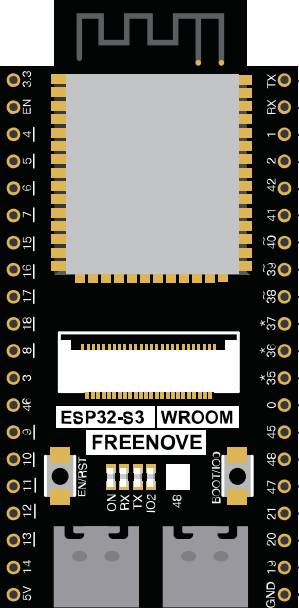
\includegraphics[width=0.22\linewidth]{freenove.png}
    \caption{Freenove ESP32-S3 Board with Integrated Camera Module}
    \label{fig:esp32_s3_board}
\end{figure}

The camera is streamed at QVGA ($320 \times 240$) resolution to keep the wireless link within
budget. This is well below the sensor's native capability and is reported here because the accuracy
of landmark-derived quantities depends on it. In particular, the camera-based distance estimate
(Section~\ref{subsec:vision}) uses a scale factor expressed in pixel units and is therefore
resolution-dependent: changing the capture source invalidates the calibration, which is why
calibration is a mandatory step rather than an optional refinement.

\subsubsection{Multimodal Physical Telemetry Sensors}
\begin{itemize}
    \item \textbf{Eye-to-Screen Distance Telemetry:} An Ultrasonic Sensor (HC-SR04) mounted
    adjacent to the monitor measures real-time distance ($Z_{\text{ultra}}$ in $\text{cm}$) between
    the user and the workstation screen \cite{cvs_distance}.
    \item \textbf{Workspace Illuminance Monitoring:} A Light Dependent Resistor (LDR) module
    collects ambient workspace illuminance levels ($L_{\text{ambient}}$ in $\text{Lux}$)
    \cite{workspace_lighting}.
\end{itemize}

Distance is therefore observed through \emph{two independent channels}: the ultrasonic rangefinder
and the camera-based estimate. This is a cross-validation arrangement rather than redundancy. The
ultrasonic sensor provides a scale reference that does not depend on image geometry, and remains
available when no face is detected; the camera estimate provides continuity when the ultrasonic
returns no echo. The two do not measure the same point --- the rangefinder returns the nearest
surface within its cone, typically the face or chest plane, whereas the camera estimate is
referenced to the interpupillary line --- so their agreement bounds precision rather than
establishing accuracy.

The illuminance channel converts the raw 12-bit ADC reading to lux by inverting the voltage divider
to the photoresistor's own resistance and applying the power-law characteristic of a CdS cell,
which is a straight line in log--log space. Two reference points fully determine that line. The
coefficients used in this work are nominal rather than measured against a photometric reference,
and the consequences are stated in Section~\ref{sec:limitations}.

\subsection{Computer Vision and Ocular Telemetry Pipeline}
\label{subsec:vision}

Instead of on-device embedded neural networks, the vision pipeline leverages a client-side computer
vision stream built on \textbf{MediaPipe} \cite{mediapipe} for spatial posture estimation and
ocular fatigue analysis.

\begin{figure}[!ht]
    \centering
    
\includegraphics[width=0.25\linewidth]{ypr.png}
    \caption{Facial Coordinate Frame Definition for Yaw ($\theta_y$), Pitch ($\theta_p$), and Roll
    ($\theta_r$). Positive pitch corresponds to the head rotating downward toward the desk.}
    \label{fig:ypr_angles}
\end{figure}

\subsubsection{3D Head Pose Estimation via MediaPipe Face Mesh}

\begin{enumerate}
    \item \textbf{Landmark Extraction:} MediaPipe Face Mesh extracts 468 3D facial keypoints from
    the camera feed in real time \cite{mediapipe}.
    \item \textbf{Perspective-n-Point (PnP) Alignment:} Selected 2D landmark coordinates (nose tip,
    chin, outer eye corners, mouth corners) are projected onto a standard 3D facial model using
    OpenCV's \texttt{solvePnP} algorithm \cite{pnp_headpose}.
    \item \textbf{Euler Angle Derivation:} The resulting rotation matrix yields the three canonical
    head orientation angles: Pitch ($\theta_p$), Yaw ($\theta_y$), and Roll ($\theta_r$).
\end{enumerate}

The reported angles are expressed \emph{relative to a per-user zero reference} captured during a
short calibration step at the start of each session, not relative to an anatomical axis. A value of
$\theta_p = 0$ therefore means ``the orientation this user adopted when asked to sit neutrally'',
not ``the cervical spine is in neutral alignment''. This choice follows the personal-calibration
approach reported for webcam posture systems \cite{ref19} and is what makes the angles comparable
within a session; its consequences for interpretation are addressed in
Section~\ref{sec:limitations}.

\subsubsection{Ocular Fatigue \& Blink Frequency Analysis (EAR)}
Visual fatigue is evaluated by computing the Eye Aspect Ratio ($EAR$) using six facial landmarks
per eye \cite{ear_blinking}:

\begin{equation}
EAR = \frac{\|p_2 - p_6\| + \|p_3 - p_5\|}{2 \|p_1 - p_4\|}
\label{eq:ear}
\end{equation}

A blink event is logged when $EAR$ falls below a threshold of $0.294$ for three consecutive frames.
This operating point differs from values commonly quoted in the literature because the magnitude of
Equation~\ref{eq:ear} depends on which landmark indices form the ratio; the present pipeline uses a
specific six-point subset per eye, and the threshold was tuned empirically for that subset rather
than inherited. Blink events are accumulated over a \emph{sliding 60-second window} to yield the
real-time blink rate in blinks per minute, with a warm-up correction of $n/t \times 60$ during the
first minute of a session so that the reported rate reflects current behaviour rather than a
cumulative average.

\subsection{From Signals to Qualified Ergonomic States}
\label{subsec:qualification}

The fused state is expressed as the feature vector $X = [P, D, L, T]$, where $P$ denotes postural
orientation, $D$ viewing distance, $L$ ambient illuminance, and $T$ cumulative exposure. Rather
than mapping $X$ to a single mutually exclusive posture label, the system evaluates each signal
independently and produces a \emph{set} of named flags. This matters because the situations the
system is intended to distinguish are precisely those in which several factors coincide: sitting
close to the screen in a dimly lit room is a different ergonomic condition from either factor
alone, and an exclusive classifier discards exactly that information.

\begin{table}[htbp]
\centering
\caption{Flag vocabulary. Flags in the danger set $D$ qualify after a shorter hold time and are
sufficient on their own to raise the alert tier.}
\label{tab:flags}
\begin{tabular}{@{}llp{6.6cm}@{}}
\toprule
\textbf{Flag} & \textbf{Set} & \textbf{Condition} \\
\midrule
\texttt{head\_too\_low}    & danger & $\theta_p > +5^\circ$ (head rotated down toward the desk) \\
\texttt{head\_too\_high}   & danger & $\theta_p < -5^\circ$ \\
\texttt{head\_tilted}      & danger & $|\theta_r| > 15^\circ$ \\
\texttt{critically\_close} & danger & Viewing distance below $30\,\text{cm}$ \\
\texttt{head\_turned}      & notice & $|\theta_y| > 20^\circ$ \\
\texttt{too\_close}        & notice & Viewing distance below $50\,\text{cm}$ \\
\texttt{too\_far}          & notice & Viewing distance above $70\,\text{cm}$ \\
\texttt{too\_dark}         & notice & Illuminance below $300\,\text{lx}$ \\
\texttt{too\_bright}       & notice & Illuminance above $500\,\text{lx}$ \\
\texttt{low\_blink\_rate}  & notice & Blink rate below $6\,\text{min}^{-1}$ \\
\bottomrule
\end{tabular}
\end{table}

Let $F(t)$ be the set of flags whose condition holds at time $t$:

\begin{equation}
F(t) = \{\, f : \text{condition}_f \text{ holds at } t \,\}
\label{eq:flags}
\end{equation}

A threshold crossing alone is not treated as an ergonomic exposure. Glancing down at the keyboard
produces a momentary crossing that is not equivalent to the same posture sustained for minutes, a
distinction the epidemiological evidence on static loading makes explicitly \cite{ref2,ref12,ref18}.
Each flag must therefore \emph{persist} for a minimum hold time $\tau_f$ before it qualifies:

\begin{equation}
Q(t) = \{\, f \in F(t) : \text{hold}_f(t) \geq \tau_f \,\}
\label{eq:qualify}
\end{equation}

where $\text{hold}_f(t)$ is the elapsed time since flag $f$ last became continuously true, and
$\tau_f$ is $15\,\text{s}$ for the danger set and $60\,\text{s}$ otherwise. The qualified set $Q(t)$
is then mapped to a severity tier:

\begin{equation}
S(t) =
\begin{cases}
\text{escalated} & \text{if the alert tier has held for } \geq 300\,\text{s} \\
\text{alert}     & \text{else if } Q \cap D \neq \emptyset \ \text{ or } \ \texttt{too\_close} \in Q \ \text{ or } \ |Q| \geq 2 \\
\text{notice}    & \text{else if } |Q| = 1 \\
\text{normal}    & \text{otherwise}
\end{cases}
\label{eq:severity}
\end{equation}

The $|Q| \geq 2$ clause is what operationalises the multimodal argument: two individually mild
conditions occurring together are treated as more serious than either alone, without requiring a
trained model to say so.

Postural variables not represented in Table~\ref{tab:flags} were excluded deliberately.
Forward-head displacement, trunk flexion, and slouching are rated of limited feasibility for a
front-facing monocular camera in Table~\ref{tab:posture_variables_detail}, and including them would
have meant reporting quantities the sensing arrangement cannot support.

\subsection{Session Lifecycle and Exposure Measurement}
\label{subsec:session}

Cumulative exposure is only a meaningful variable if it measures time the user actually spent at
the desk. Monitoring is therefore scoped to an explicit session with the states
\textit{idle}, \textit{calibrating}, \textit{monitoring}, \textit{away}, \textit{break}, and
\textit{ended}. Three rules govern the exposure clock:

\begin{itemize}
    \item Exposure accumulates \textbf{only} in the \textit{monitoring} state with a face detected
    --- not merely while the application is open.
    \item Loss of face detection for $30\,\text{s}$ moves the session to \textit{away} and
    \textbf{pauses} the clock. Returning within $180\,\text{s}$ resumes the accumulated total;
    beyond that the exposure counter restarts. A naive timer would otherwise either reset on every
    dropped frame or continue counting an empty chair.
    \item A $20\,\text{s}$ grace period after session start excludes settling-in samples, and those
    samples are marked so that they are also excluded from session-level aggregates.
\end{itemize}

An idle session closes automatically after $900\,\text{s}$ without the user returning. The exposure
measured under these rules is \emph{continuous uninterrupted desk exposure}, which is the quantity
relevant to break-taking guidance. It is not an estimate of daily cumulative sedentary load, and no
claim is made that it maps onto the daily-duration odds ratios reported in Section~\ref{sec:litreview}.

\subsection{Notification Governor}
\label{subsec:governor}

Detecting an unfavourable condition and interrupting the user are different decisions. A system
that raises an alert on every qualified state produces the repetitive generic warnings criticised
in Section~\ref{sec:litreview}, and the practical consequence is that users disable it. The
governor sits between qualification and delivery and applies four rules:

\begin{itemize}
    \item \textbf{Deduplication.} The invocation key is the qualified flag set itself. A condition
    that persists unchanged does not generate a new explanation; a change in the set does.
    \item \textbf{Exponential backoff.} If the same condition remains uncorrected, reminders are
    repeated on a lengthening schedule rather than at a fixed interval. The backoff resets once the
    state has been normal for $120\,\text{s}$, so a later, unrelated violation is still raised
    promptly.
    \item \textbf{Escalation.} An alert sustained for $300\,\text{s}$ escalates and requires
    explicit acknowledgement, which is the design's position on alert fatigue: rather than
    increasing frequency, the system increases salience once and then waits.
    \item \textbf{User control.} Snooze suppresses reminders for $600\,\text{s}$ and a
    do-not-disturb mode suppresses them indefinitely, both reversible from the dashboard.
\end{itemize}

Governor state is persisted with the session record, so cooldowns survive a restart or a second
open dashboard rather than resetting --- without this, a page reload would silently re-enable an
alert the user had just dismissed.

Each delivered reminder additionally opens a $60\,\text{s}$ observation window and records whether
the triggering flags cleared within it. This yields a corrected-per-reminder ratio per session and
is the instrument for the behavioural question posed in Section~\ref{sec:protocol}.

\subsection{Feedback and Intervention Channels}
\label{subsec:feedback}

Interventions are delivered through three channels:

\begin{itemize}
    \item \textbf{Device indication.} The ESP32-S3 drives a two-colour indicator from a state
    object in the Realtime Database: green while monitoring normally, red at the alert tier, and
    blinking red when escalated. Fetching and blinking are non-blocking so that camera streaming
    and sensor sampling are unaffected.
    \item \textbf{Speech.} A single-sentence spoken form of the recommendation is delivered through
    browser speech synthesis. It is opt-in and enabled during guided setup.
    \item \textbf{Interface.} A transient notification carries the governor's available actions
    (snooze, do-not-disturb, acknowledge). A break suggestion is raised when continuous exposure
    reaches its threshold, and is synchronised bidirectionally with the built-in focus timer so
    that a timed break also suspends posture alerting.
\end{itemize}

\subsection{Cloud LLM Integration and Ergonomic Reasoning}
\label{subsec:llm}

The role of the language model \cite{llm_reasoning} is to translate a measured state into an
explanation, not to detect, diagnose, or decide when to interrupt --- those decisions are made by
the deterministic layers above. Invocation is \emph{event-driven}: a request is issued when the qualified flag set
changes, not on a timer. The distinction is material to deployment cost. At the backend's
$10\,\text{s}$ sampling interval, a periodic design would issue on the order of $360$ requests per
hour of sustained poor posture, whereas the governor issues one per distinct condition plus
scheduled repetitions under backoff.

Two bounded prompt modes are used. In \textit{advice} mode the model is constrained to the detected
flags and asked to explain why that combination is unfavourable and what to adjust. In
\textit{explain} mode, used when the user requests an assessment while all readings are in target,
the model is explicitly instructed not to invent a problem. Output follows a fixed
Context/Advice/Spoken contract, the third field being the single short sentence used for speech.

When the API is unavailable the system falls back to a deterministic per-flag phrase table and
labels the resulting record accordingly, so that non-generated text is distinguishable in the logs.

\subsection{Data Schema and Operating Parameters}
\label{subsec:schema}

Table~\ref{tab:data_variables} lists the variables recorded for each sample, and
Table~\ref{tab:parameters} the operating parameters that govern how they are interpreted.

\begin{table}[htbp]
\centering
\caption{Multimodal data variables and system roles}
\label{tab:data_variables}
\begin{tabular}{@{}llp{7.2cm}@{}}
\toprule
\textbf{Variable} & \textbf{Type} & \textbf{Description / Ergonomic Significance} \\
\midrule
Session\_ID        & Categorical & Identifier scoping all rows to one monitoring session \\
Timestamp          & Time        & UNIX timestamp for multi-sensor stream synchronisation \\
State              & Categorical & Session state (idle, calibrating, monitoring, away, break, ended) \\
$\theta_p, \theta_y, \theta_r$ & Continuous & Head orientation Euler angles in degrees ($^\circ$), relative to the calibrated zero \\
EAR                & Continuous & Instantaneous Eye Aspect Ratio \\
Blink Rate         & Continuous & Blink frequency over a sliding 60-second window ($\text{min}^{-1}$) \\
Distance (camera)  & Continuous & Interpupillary-distance estimate of user-to-screen distance (cm) \\
Distance (ultrasonic) & Continuous & Independently measured user-to-screen distance (cm) \\
Light Reading      & Continuous & Workspace ambient illuminance (Lux), with a range status flag \\
Face Present       & Boolean    & Whether a face was detected; gates exposure accumulation \\
Exposure           & Continuous & Continuous uninterrupted desk exposure (s) \\
Flag Set           & Set        & Conditions currently true (Table~\ref{tab:flags}) \\
Flag Durations     & Continuous & Per-flag persistence used by Equation~\ref{eq:qualify} \\
Severity           & Categorical & Tier assigned by Equation~\ref{eq:severity} \\
Reminders / Corrected & Integer & Interventions delivered, and those followed by a correction \\
\bottomrule
\end{tabular}
\end{table}

All operating parameters are read from a single configuration file, so that the values below are
the values the running system uses. Table~\ref{tab:parameters} lists them in full to support
replication.

\begin{table}[htbp]
\centering
\caption{Operating parameters as configured}
\label{tab:parameters}
\begin{tabular}{@{}llp{6.4cm}@{}}
\toprule
\textbf{Parameter} & \textbf{Value} & \textbf{Role} \\
\midrule
\multicolumn{3}{@{}l}{\textit{Detection thresholds}} \\
Pitch                & $\pm 5^\circ$              & Head down / back from calibrated zero \\
Roll                 & $\pm 15^\circ$             & Lateral head tilt \\
Yaw                  & $\pm 20^\circ$             & Rotation away from the screen \\
Viewing distance     & $50$--$70\,\text{cm}$      & Target range \\
Distance, critical   & $< 30\,\text{cm}$          & Distinct acute band \\
Illuminance          & $300$--$500\,\text{lx}$    & Workspace ambient target \\
Blink rate           & $\geq 6\,\text{min}^{-1}$  & Sliding 60\,s window \\
EAR                  & $0.294$ / 3 frames         & Blink event threshold and debounce \\
\midrule
\multicolumn{3}{@{}l}{\textit{Temporal qualification} ($\tau_f$)} \\
Danger flags         & $15\,\text{s}$             & Head-pose and critically-close hold \\
Notice flags         & $60\,\text{s}$             & Lighting, blink rate, distance, head turned \\
Escalation           & $300\,\text{s}$            & Sustained alert without correction \\
\midrule
\multicolumn{3}{@{}l}{\textit{Notification governor}} \\
Backoff              & $60$, $180\,\text{s}$      & Repeat schedule for an unchanged condition \\
Snooze               & $600\,\text{s}$            & User-initiated suppression \\
Normal reset         & $120\,\text{s}$            & Clear time before backoff returns to first step \\
Correction window    & $60\,\text{s}$             & Observation window after a reminder \\
\midrule
\multicolumn{3}{@{}l}{\textit{Session}} \\
Grace                & $20\,\text{s}$             & Post-start settling, excluded from aggregates \\
Face lost $\to$ away & $30\,\text{s}$             & Pause exposure accumulation \\
Away $\to$ reset     & $180\,\text{s}$            & Beyond this, exposure restarts \\
Idle $\to$ end       & $900\,\text{s}$            & Auto-close the session \\
Break suggestion     & $1200\,\text{s}$           & Continuous exposure trigger \\
Sampling interval    & $10\,\text{s}$             & Backend; vision pipeline runs at $\approx$6--7\,Hz \\
\bottomrule
\end{tabular}
\end{table}





\section{Conclusion}
Your conclusion here

\section*{Acknowledgments}
This was was supported in part by......

%Bibliography
\bibliographystyle{unsrt}  
\bibliography{references}  


\end{document}
